\chapter{Các công trình liên quan}
\label{Chapter2}

\section{Gom nhóm phân cấp}
\subsection{Giới thiệu}
%Giới thiệu phương pháp gom nhóm phân cấp
Gom nhóm phân cấp là phương pháp gom nhóm dùng để xây dựng các nhóm thành các cấp bậc khác nhau.
Các phương pháp gom nhóm được liệt kê ở chương 1 cho ta thấy được sự hiệu quả trong việc gom nhóm và tương đối đơn giản.
Tuy nhiên, các phương pháp này chỉ cho ta thấy được kết quả gom nhóm cuối cùng, không cho chúng ta thấy được cấu trúc của dữ liệu.
Hơn thế nữa, các phương pháp này đa phần cần phải xác định số lượng phân nhóm ban đầu.
Vì vậy, một phương pháp khác được giới thiệu là gom nhóm phân cấp để khắc phục các nhược điểm trên.

\subsection{Các hướng tiếp cận}
%Các hướng tiếp cận
Để xây dựng nên cấu trúc cây của các phân nhóm trong gom nhóm phân cấp, ta có hai hướng tiếp cận khác nhau. Đó là hướng tiếp cận tích tụ và hướng tiếp cận phân chia.

	\subsubsection{Hướng tiếp cận tích tụ}
	%Hướng tiếp cận agglomerative
		%Giới thiệu
		Hướng tiếp cận tích tụ là một trong những cách tiếp cận của gom nhóm phân cấp.
		Đây là phương pháp tiếp cận gom nhóm theo cách đi từ dưới lên.
		Phương pháp này bắt đầu từ việc quan sát mỗi phân nhóm, các phân nhóm sẽ gom lại với nhau và chuyển thành cấp cao hơn trong cây.
		Trong trường hợp thông thường, độ phức tạp của thuật toán theo hướng tiếp cận tích tụ là $O(n^2\log(n))$.
		Tuy nhiên, thuật toán có thể tối ưu hóa để làm giảm độ phức tạp bằng cách sử dụng liên kết đơn hoặc là liên kết toàn phần.
		
		%Ví dụ
		Cho dữ liệu thô sau, ta sẽ sử dụng hướng tiếp cận tích tụ để gom nhóm phân cấp với công thức tính khoảng cách là Euclid.
		
		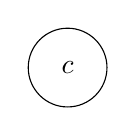
\begin{tikzpicture}
		\draw(10,20) circle (5mm) node{$c$};
		\end{tikzpicture}
	
	\subsubsection{Hướng tiếp cận phân chia}
	%Hướng tiếp cận divisive	
		%Giới thiệu
		Hướng tiếp cận phân chia là một trong những cách tiếp cận của gom nhóm phân cấp.
		Đây là phương pháp tiếp cận gom nhóm theo cách đi từ trên xuống.
		Phương pháp này bắt đầu từ việc quan sát tất cả chỉ trong một phân nhóm, và khi di chuyển xuống sẽ tách dần dần thành các phân nhóm con.
		Quá trình gộp và tách thường sẽ tốn nhiều chi phí cho thuật toán.
		Khác với hướng tiếp cận tích tụ, hướng tiếp cận phân chia có độ phức tạp lớn hơn, $O(2^n)$.
		
		%Ví dụ
		
%Các công thức tính khoảng cách
%Trong gom nhóm văn bản, các công thức tính khoảng cách được sử dụng để đo lường giữa hai văn bản. Sau đây, một số công thức tính khoảng cách thường được sử dụng:
%\begin{enumerate}
%\item[•]Khoảng cách Euclidean : $\parallel a \,- \, b \parallel_2 \, = \, \sqrt{\underset{i}{\sum}(a_i \, - \, b_i)^2} $
%\item[•]Khoảng cách Euclidean vuông : $\parallel \, a \, - \, b \, \parallel^2_2 \, = \, \underset{i}{\sum} (a_i - b_i)^2$
%\item[•]Khoảng cách Manhatthan : $\parallel \, a \, - \, b \, \parallel_1 \, = \, \underset{i}{\sum} \mid a_i \, - \, b_i\mid$
%\item[•]Khoảng cách cực đại : $\parallel \, a \, - \, b\, \parallel_\infty \, = \, \underset{i}{max} \mid a_i \, - \, b_i \mid$
%\item[•]Khoảng cách Mahalanobis : $\sqrt{(a \, - \, b)^{\top} \, S^{-1} \, (a \, - \, b)}$ với $S$ là ma trận covariance
%\end{enumerate}

%Các phương pháp liên kết trong hướng tiếp cận tích tụ
\subsection{Các phương pháp liên kết trong hướng tiếp cận tích tụ}
		
%Đồng gom nhóm phân cấp
\section{Đồng gom nhóm phân cấp}

	%Giới hạn của gom nhóm
	\subsection{Giới hạn của gom nhóm}
	
	%Giới thiệu đồng gom nhóm
	\subsection{Giới thiệu đồng gom nhóm}
	Đồng gom nhóm là phương pháp gom nhóm cả hai chiều của dữ liệu(bao gồm gom nhóm văn bản và gom nhóm đặc trưng).
	Đây là phương pháp hiệu quả vì khai thác được độ tương đồng của các phân nhóm trong chiều này của dữ liệu để gom nhóm trong chiều khác.
	Điều này có nghĩa các phân nhóm của văn bản được đánh giá bằng các phân nhóm của đặc trưng và ngược lại.
	Bằng cách này, các phân nhóm của văn bản có thể được tiến hành dựa trên các phân nhóm đặc trưng để giúp làm giảm số chiều của dữ liệu.
	Như vậy, đồng gom nhóm là phương pháp hữu hiệu để giúp ta gom nhóm văn bản đồng thời làm giảm số chiều của dữ liệu.
	%Ví sao chọn đồng gom nhóm
	%Lợi ích của đồng gom nhóm
	%Sự kết hợp của đồng gom nhóm với gom nhóm phân cấp
	%Công dụng của đồng gom nhóm phân cấp
	%Lợi ích của đồng gom nhóm phân cấp
	%Giải thích việc tương tác hai chiều dữ liệu
	%Kết luận về đồng gom nhóm phân cấp

%%14

%Độ tương đồng Goodman kruskal
\section{Độ tương đồng Goodman kruskal}

	\subsection{Contingency table}
	%Giới thiệu về contingency table
	%Ví dụ về contingency table
	
	\subsection{Độ tương đồng Goodman Kruskal}
	%Giới thiệu về độ tương đồng Goodman Kruskal
	%Vì sao chọn độ tương đồng Goodman Kruskal
	%Sử dụng Goodman kruskal trong đồng gom nhóm phân cấp
	%Luật sử dụng cho độ tương đồng Goodman kruskal
		%Giới thiệu
		%Luật thứ nhất
		%Luật thứ hai
	%Ví dụ về cách tính Goodman kruskal
	%Cách để gom nhóm những hàng với nhau
	%Cách để gom nhóm những cột với nhau
%%11

%Thuật toán đồng gom nhóm phân cấp
\section{Thuật toán đồng gom nhóm phân cấp}
	%Các ý cần giải thích
	\subsection{Các ý cần giải thích}
		%Dòng, cột, ma trận trong thuật toán(2 đoạn)
		%Mục tiêu của đồng gom nhóm phân cấp
		%Điều kiện của các nhóm trong hàng, cột
		%Cách để gom lại các nhóm trong ma trận
		%Cách để tạo ra phân nhóm đầu tiên(2 đoạn)
	%%7
	
	\subsection{Áp dụng Goodman kruskal trong đồng gom nhóm phân cấp}
	%Sử dụng Goodman kruskal trong đồng gom nhóm phân cấp
	
		%Giới thiệu
		\subsubsection{Giới thiệu}		
		
		%Công thức
		\subsubsection{Công thức}
		
		%Ý tưởng
		\subsubsection{Ý tưởng}
			%Định nghĩa một
			%Định nghĩa hai
		%Giải thích
		%Cách áp dụng để tính nhóm thích hợp
		%Giải thích cách tính	
		%Sự tối ưu hóa của cách tính
		%Sự lựa chọn nhóm được gom
		%kết quả cuối cùng khi áp dụng
		%kết luận
	%%11
	%Thuật toán
	\subsection{Thuật toán}
		%Giải thuật 1
		%Giải thuật 2
		%Giải thuật 3
		%Giải thuật 4
		%Giải thích toàn bộ giải thuật của thuật toán(15 đoạn)
	%%19
	
	%Những lưu ý về đồng gom nhóm phân cấp
	\subsection{Những lưu ý về đồng gom nhóm phân cấp}
		%Các tác động đến đồng góm nhóm phân cấp
		%Sự ảnh hưởng của từng tác động này(6 đoạn)
	%%7
%%44
		
%Đồng gom nhóm phân cấp theo hướng tăng trưởng
\section{Đồng gom nhóm phân cấp theo hướng tăng trưởng}
	%Điểm hạn chế hiện thời của đồng gom nhóm phân cấp
	%Phân tích tình huống của thuật toán hiện thời
	%Phát triển thuật toán cho dữ liệu tăng trưởng theo thời gian thực
	%hướng cần phải giải quyết
	%Các giải thuật
		%Giải thuật 5
		%Giải thuật 6
	%Giải thích các giải thuật theo hướng tổng quát(15 đoạn)
%%21
%%90	


%%%%%%%%%%%%%%%%%%%%%%%%%%%%%%%%%%%%%%%%%%%%%%%%%%%%%%%%%%%%%%%%%%55
%\section{Các phương pháp gom nhóm}
%%kể ra một vài phương pháp gom nhóm: kmeans, DBScan
%
%\section{Phương pháp gom nhóm phân cấp}
%\subsection{Các hướng tiếp cận}
%\subsubsection{Hướng tiếp cận agglomerative}
%%Giới thiệu hướng tiếp cận agglomerative
%
%%Ví dụ về agglomerative
%
%\subsubsection{Hướng tiếp cận divisive}
%%Giới thiệu hướng tiếp cận divisive
%
%%Ví dụ về divisive
%
%\section{Đồng gom nhóm phân cấp}
%\subsection{Giới thiệu}
%%Điểm hạn chế về gom nhóm
%
%%Giới thiệu về đồng gom nhóm
%
%%Sự kết hợp của đồng gom nhóm phân cấp
%
%%Công dụng của đồng gom nhóm phân cấp
%
%%Giải thích việc tương tác hai chiều của dữ liệu
%
%%Kết luận về đồng gom nhóm phân cấp
%
%\subsection{Độ tương đồng Goodman Kruskal $\tau$}
%%Vì sao chọn Goodman Kruskal $\tau$
%
%%Giới thiệu Goodman Kruskal $\tau$
%
%%Luật sử dụng Goodman Kruskal $\tau$
%
%%Ví dụ về Goodman Kruskal
%
%\subsection{Thuật toán}
%%Giới thiệu thuật toán
%
%%Các giải thuật
%
